\chapter{图像有损压缩实验结果}

\section{实验结果的定性分析}
\begin{figure}
    \centering
    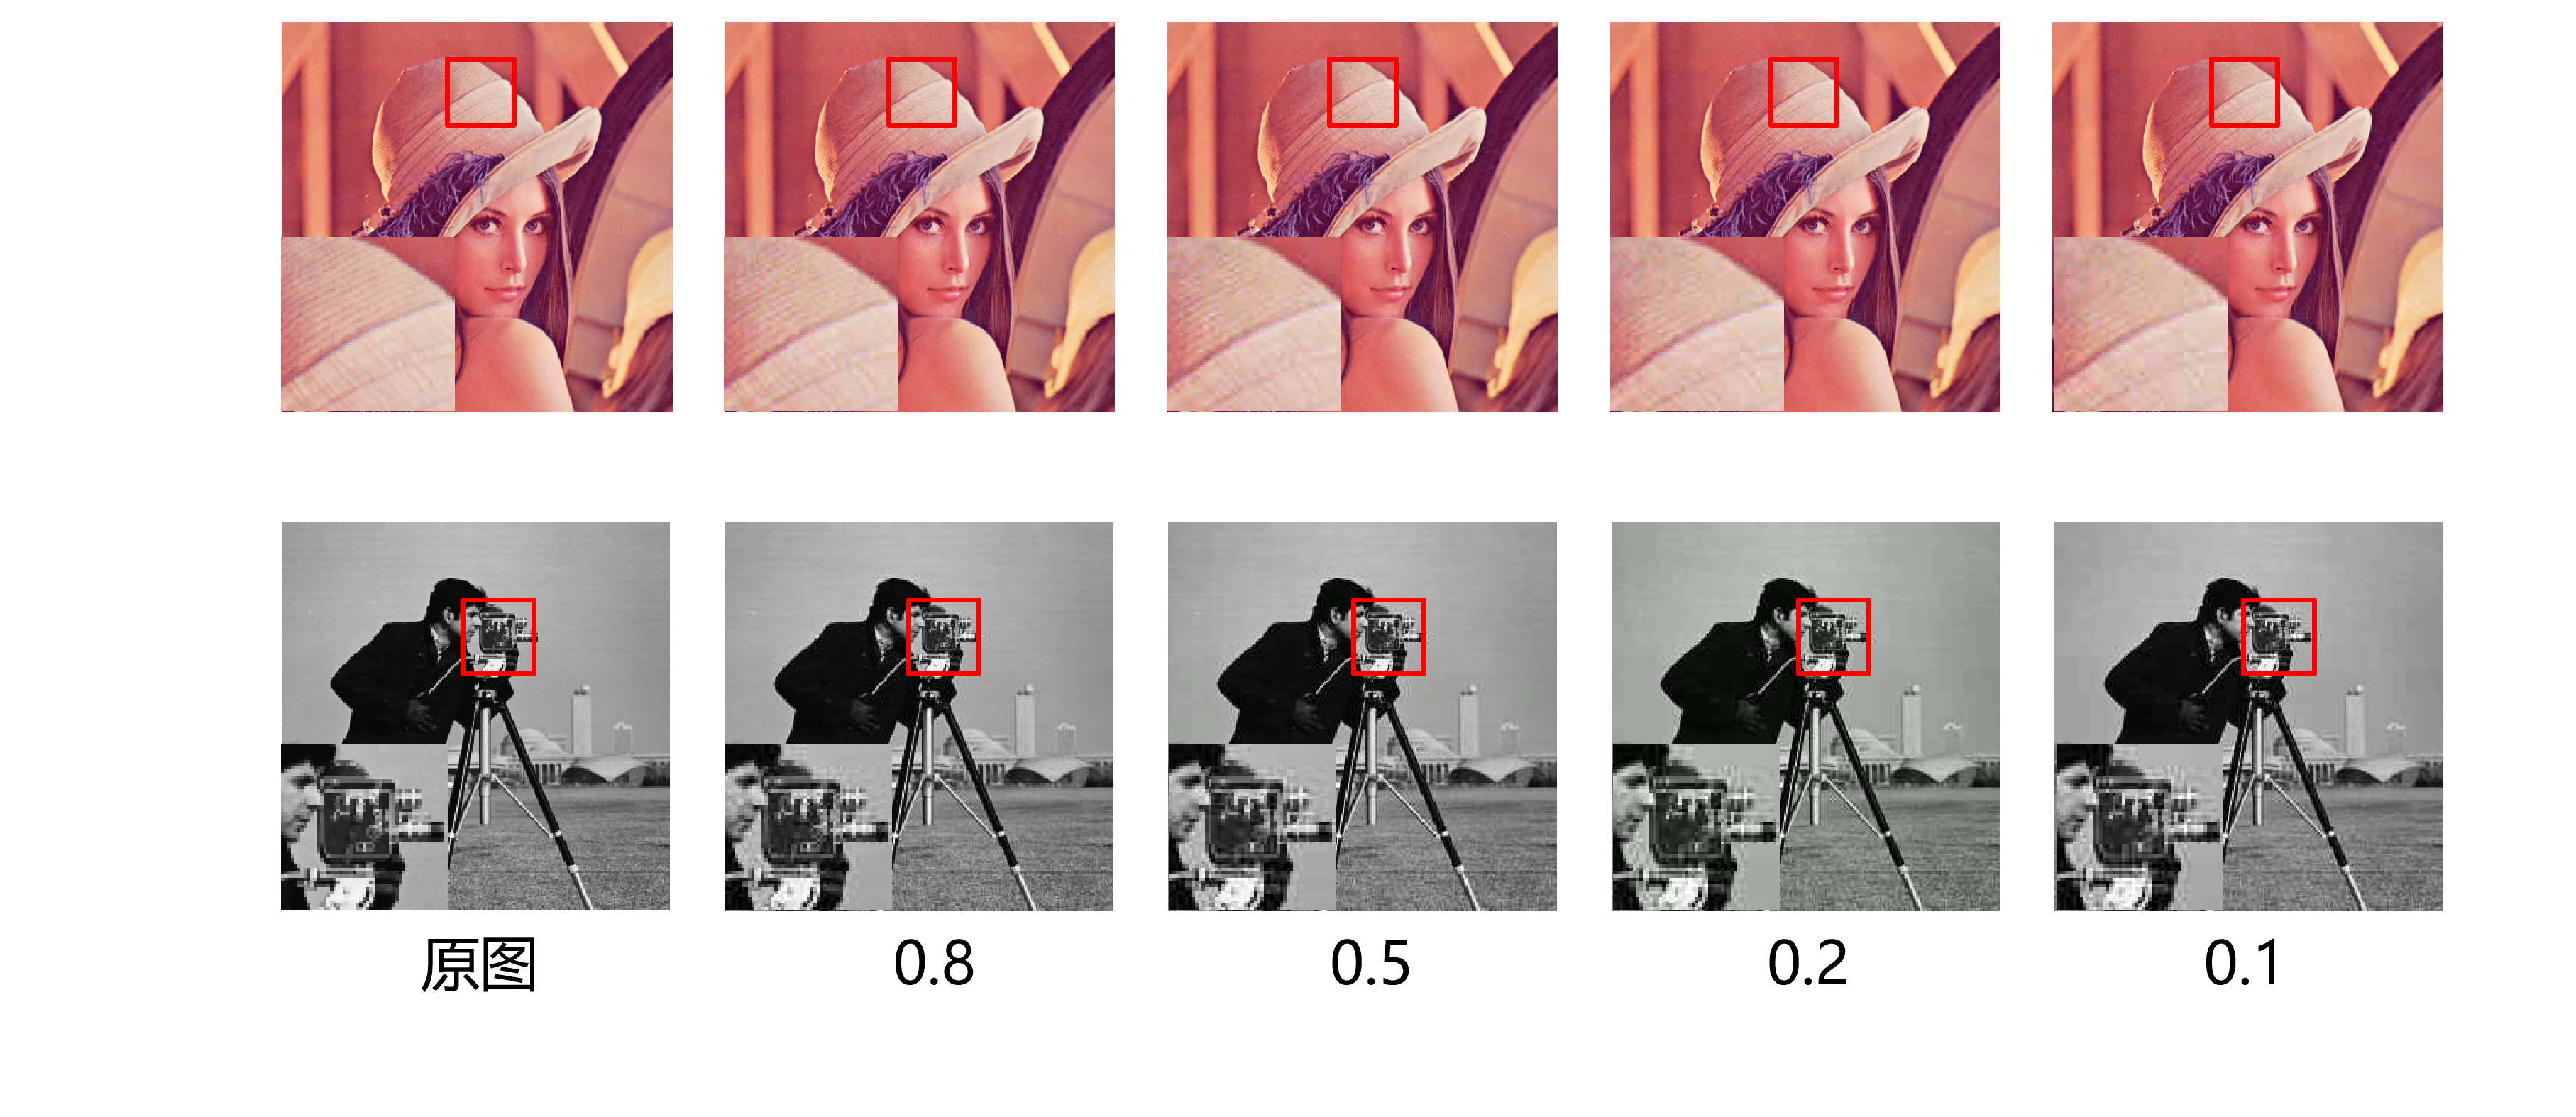
\includegraphics[width=1.0\textwidth]{pages/evaluation/result-image.png}
    \caption{实验结果的定性分析}
    \label{Fig.result}
\end{figure}

\section{实验结果的定量分析}
\subsection{性能指标}

\subsubsection{MSE}
均方误差(MSE)定义为原图各像素$I(i,j)$与压缩后图像各像素$K(i,j)$差的平方和(式\ref{Eq.MSE})
\begin{equation}
    MSE=\frac{1}{mn} \sum_{i=0}^{m-1}\sum_{j=0}^{n-1} [I(i,j)-K(i,j)]^2
    \label{Eq.MSE}
\end{equation}

\subsubsection{PSNR}
峰值信噪(PSNR)比定义为
\begin{equation}
    PSNR=20\lg (\frac{Max_1}{\sqrt{MSE}})
    \label{Eq.PSNR}
\end{equation}
其中$Max_1$是表示图像点颜色的最大数值,$MSE$为均方误差。


\subsubsection{SSIM}
样本$(x,y)$的结构相似度为
\begin{equation}
    SSIM(x,y)=\frac{2\mu_x\mu_y+C_1}{\mu_x^2+\mu_y^2+C_1}\cdot\frac{2\delta_{xy}+C_2}{\delta_x^2+\delta_y^2+C_2}
    \label{Eq.SSIM}
\end{equation}

\subsubsection{压缩比}

压缩比定义为原图片比特数与压缩后图片比特数之比。



\subsection{定量结果}

\begin{table}[h!]
    \begin{center}
        \caption{MSE}
        \begin{tabular}{c|ccccc}
            \textbf{压缩质量} & 0.8 & 0.5 & 0.3 & 0.2 & 0.1 \\
            \hline
            \textbf{MSE} & 4.92 & 5.40 & 5.73 & 5.90 & 6.00 \\
        \end{tabular}
    \end{center}
\end{table}


\begin{table}[h!]
    \begin{center}
        \caption{PSNR}
        \begin{tabular}{c|ccccc}
            \textbf{压缩质量} & 0.8 & 0.5 & 0.3 & 0.2 & 0.1 \\
            \hline
            \textbf{PSNR} & 41.2 & 40.8 & 40.5 & 40.4 & 40.3 \\
        \end{tabular}
    \end{center}
\end{table}

\begin{table}[h!]
    \begin{center}
        \caption{SSIM}
        \begin{tabular}{c|ccccc}
            \textbf{压缩质量} & 0.8 & 0.5 & 0.3 & 0.2 & 0.1 \\
            \hline
            \textbf{PSNR} & 0.98 & 0.98 & 0.98 & 0.98 & 0.98 \\
        \end{tabular}
    \end{center}
\end{table}



\begin{table}[h!]
    \begin{center}
        \caption{压缩比}
        \begin{tabular}{c|ccccc}
            \textbf{压缩质量} & 0.8 & 0.5 & 0.3 & 0.2 & 0.1 \\
            \hline
            \textbf{游程压缩比}     & 7.99 & 9.88 & 10.9 & 11.4 & 11.8 \\
            \textbf{总压缩比}       & 13.0 & 16.2 & 18.2 & 19.2 & 20.0 \\
            \textbf{Matlab压缩比}   & 17.8 & 32.3 & 44.5 & 56.6 & 82.2 \\
        \end{tabular}
    \end{center}
\end{table}